%%
%% This is file `sample-sigchi.tex',
%% generated with the docstrip utility.
%%
%% The original source files were:
%%
%% samples.dtx  (with options: `sigchi')
%% 
%% IMPORTANT NOTICE:
%% 
%% For the copyright see the source file.
%% 
%% Any modified versions of this file must be renamed
%% with new filenames distinct from sample-sigchi.tex.
%% 
%% For distribution of the original source see the terms
%% for copying and modification in the file samples.dtx.
%% 
%% This generated file may be distributed as long as the
%% original source files, as listed above, are part of the
%% same distribution. (The sources need not necessarily be
%% in the same archive or directory.)
%%
%% The first command in your LaTeX source must be the \documentclass command.
\documentclass[sigchi]{acmart}
\usepackage{lineno}
\usepackage{graphicx}

%%
%% \BibTeX command to typeset BibTeX logo in the docs
\AtBeginDocument{%
  \providecommand\BibTeX{{%
    \normalfont B\kern-0.5em{\scshape i\kern-0.25em b}\kern-0.8em\TeX}}}

%% Rights management information.  This information is sent to you
%% when you complete the rights form.  These commands have SAMPLE
%% values in them; it is your responsibility as an author to replace
%% the commands and values with those provided to you when you
%% complete the rights form.
\setcopyright{acmcopyright}
\copyrightyear{2018}
\acmYear{2018}
\acmDOI{10.1145/1122445.1122456}

%% These commands are for a PROCEEDINGS abstract or paper.
\acmConference[Regensburg '19]{Regensburg '19: Social Acceptance of Nomadic Virtual
  Reality }{June 02--??, 2019}{Bayern, DE}
\acmBooktitle{Regensburg '19: Social Acceptance of Nomadic Virtual
  Reality, June 02--??, 2019, Bayern, DE}
\acmPrice{00.00}

%%
%% Submission ID.
%% Use this when submitting an article to a sponsored event. You'll
%% receive a unique submission ID from the organizers
%% of the event, and this ID should be used as the parameter to this command.
%%\acmSubmissionID{123-A56-BU3}

%%
%% The majority of ACM publications use numbered citations and
%% references.  The command \citestyle{authoryear} switches to the
%% "author year" style.
%%
%% If you are preparing content for an event
%% sponsored by ACM SIGGRAPH, you must use the "author year" style of
%% citations and references.
%% Uncommenting
%% the next command will enable that style.
%%\citestyle{acmauthoryear}

%%
%% end of the preamble, start of the body of the document source.
\begin{document}

%%
%% The "title" command has an optional parameter,
%% allowing the author to define a "short title" to be used in page headers.
\title{Social Acceptance of Nomadic Virtual Reality}

%%
%% The "author" command and its associated commands are used to define
%% the authors and their affiliations.
%% Of note is the shared affiliation of the first two authors, and the
%% "authornote" and "authornotemark" commands
%% used to denote shared contribution to the research.
\author{Alexander Eder}
\email{Alexander.Eder@stud.uni-regensburg.de}
\affiliation{%
  \institution{Universität Regensburg}
  \streetaddress{Universitätsstraße 31}
  \city{Regensburg}
  \state{Deutschland}
  \postcode{93053}
}

\author{Stephan Jäger}
\email{Stephan.Jaeger@stud.uni-regensburg.de}
\affiliation{%
  \institution{Universität Regensburg}
  \streetaddress{Universitätsstraße 31}
  \city{Regensburg}
  \state{Deutschland}
  \postcode{93053}
}

\author{Tom Nedorost}
\email{Alexander-Tom.Nedorost@stud.uni-regensburg.de}
\affiliation{%
  \institution{Universität Regensburg}
  \streetaddress{Universitätsstraße 31}
  \city{Regensburg}
  \state{Deutschland}
  \postcode{93053}
}

%%
%% By default, the full list of authors will be used in the page
%% headers. Often, this list is too long, and will overlap
%% other information printed in the page headers. This command allows
%% the author to define a more concise list
%% of authors' names for this purpose.
\renewcommand{\shortauthors}{Eder and Jäger and Nedorost}
\linenumbers

%%
%% The abstract is a short summary of the work to be presented in the
%% article.
\begin{abstract}
The on hand paper provides an overview on the reviewed social acceptance of nomadic virtual reality devices in a university environment using the example oft the Oculus Rift. Within the scope of a field study data regarding fears and desires was collected with the help oft the so-called WEAR scale. Three different cases (Smartphone, Oculus Rift without gesture control, Oculus Rift with gesture control) have been reviewed. In this case the smartphone served as a comparative size due to its high acceptance as a daily used wearable. An actor and an actress that both created situations with using all of the three cases, became rated by overleaf passerbys on the basis of the above-mentioned scale in form of questionaires. The evaluation shows that virtual devices are more accepted as one thinks. The biggest difference can be found in the contemplation between smartphone and the usage of a VR device in combination with performing gestures with a VR controller. Here it becomes clear that gesture control in this context is still unfamiliar and something that makes people feel more uncomfortable compared to the handling of „ordinary“ wearables.
\end{abstract}

%%
%% The code below is generated by the tool at http://dl.acm.org/ccs.cfm.
%% Please copy and paste the code instead of the example below.
%%
\begin{CCSXML}
<ccs2012>
 <concept>
  <concept_id>10010520.10010553.10010562</concept_id>
  <concept_desc>Computer systems organization~Embedded systems</concept_desc>
  <concept_significance>500</concept_significance>
 </concept>
 <concept>
  <concept_id>10010520.10010575.10010755</concept_id>
  <concept_desc>Computer systems organization~Redundancy</concept_desc>
  <concept_significance>300</concept_significance>
 </concept>
 <concept>
  <concept_id>10010520.10010553.10010554</concept_id>
  <concept_desc>Computer systems organization~Robotics</concept_desc>
  <concept_significance>100</concept_significance>
 </concept>
 <concept>
  <concept_id>10003033.10003083.10003095</concept_id>
  <concept_desc>Networks~Network reliability</concept_desc>
  <concept_significance>100</concept_significance>
 </concept>
</ccs2012>
\end{CCSXML}

\ccsdesc[500]{Computer systems organization~Embedded systems}
\ccsdesc[300]{Computer systems organization~Redundancy}
\ccsdesc{Computer systems organization~Robotics}
\ccsdesc[100]{Networks~Network reliability}

%%
%% Keywords. The author(s) should pick words that accurately describe
%% the work being presented. Separate the keywords with commas.
\keywords{virtual reality, social acceptance, nomadic, field study}


%%
%% This command processes the author and affiliation and title
%% information and builds the first part of the formatted document.
\maketitle

\section{Introduction}
New presentation methods such as VR experiences are a growing trend as alternatives to conventional screens in different end devices for example tablets or mobile phones. These devices are always improving in measurements, functionality, and appearance because of this trend, to accommodate the mobility of modern life. Due to this development process never standing still VR devices might be prospectively used in the same way we already use mobile phones today, at any time and everywhere. To achieve a broad utilization, it is not only important to focus on the unique user and establish hardware with high usability for the users themselves, but also something that fits all the tangentially involved people and their needs for well-being, comfort, and privacy. The most important issue to start with, which also is the topic of this paper, is the question about the current state of social acceptance of VR devices in public spaces. Before spreading out this type of gear and gaining the possibility of high sales output it is essential to find out if those devices are already accepted by society and which impacts they have on society.

 \cite{schwind2018virtual} Several researchers already tried to investigate this potential issues regarding the social acceptance by showing pictures and videos of people wearing VR devices in public spaces to a group of test persons under laboratory conditions to find out more about their opinions, feelings, and reactions confronted with this subject.  With the inspection of images, people will always keep a certain emotional distance to the context shown. 
The spontaneous confrontation with a previously completely unexpected situation in daily life might have another effect on their emotional acceptance. VR devices might be fully accepted by society, but it can also be that they evoke discomfort because people are not used to not seeing each other's eyes while passing by or sitting next to them on the bench. Sunglasses of course act similar but since today´s VR glasses still cover almost half of the wearers face it cannot be generalized and needs to be examined more accurately.
In this paper, we reexamined the topic of social acceptance of VR devices using a field study to achieve a high validity.

\section{Related Work}
Previous work already dealt with social acceptance and mobile devices. Gesture control has also been investigated. In the following, three papers will be analysed that already tried to gather information about how devices of that kind are accepted in a social context.

One work dealing with gesture control and mobile devices and their social acceptance is a work by J. Rico and S. Brewster \cite{rico2010usable}. It mainly observes the extent to which social acceptance can be measured. They found out that the social acceptance of technology use is not just a question of embarrassment or politeness, but a combination of factors ranging from appearance and social status to culture. It was also stressed that gesture-based user interfaces face acceptance problems as they require users to evaluate a range of new actions. This would require the user to define new standards for social acceptance. In a survey, they found that location and audience have a significant impact on whether a user wants to perform gestures. For example, a user would be more likely to make gestures in front of trusted people. This led to the conclusion that users would be more likely to use gesture-controlled mobile devices at home. Two other areas that were defined were the semi-public space, i.e. with a restricted but not necessarily familiar audience, and the public space, i.e. the sidewalk. They then carried out another experiment to see how participants behave when they make gestures on a busy street. Since this work is not about the design question, the last attempt is negligible.

The paper "Understanding the Social Acceptability of Mobile Devices using the Stereotype Content Model" \cite{schwind2019understanding} criticized that there was no robust model to explain  the underlying factors why a device was socially acceptable. Therefore, the devices were regarded as social objects and it was examined whether the stereotypical content model (SCM) could be applied to them. The focus of this work was clearly on whether mobile applications in themselves meet a stereotype. This has been proven in two studies. In the first study it was found that different devices have a different impact on the person wearing them. LED glasses, for example, were viewed negatively. In the work, this was associated with low warmth and low competence. Medical devices, on the other hand, were rated more positively or warmer. VR headsets were rated well in terms of being more competitive, but they overall were received as contemptous. It was also found that devices systematically trigger emotions when people use them. This may allow the SCM to explain the results of older work, as the social acceptance of highly competitive devices such as smart glasses depends on the stereotype of the person wearing the device. Here the comparison was made between older people wearing a VR headset and other people. A weaker attraction was also measured for VR glasses than for other devices. It can therefore be assumed that the SCM can be used to measure the social acceptance of a mobile device. These assumptions were confirmed in a second study. In this study no images of human stereotypes were used and since it showed no significant difference to the stereotype device combinations of the first study, it was assumed that a possible effect of human stereotype images is negligible. In addition, it was proven once again that VR glasses are assigned a certain competence and that they are perceived more competitively.

Schwind et al investigated the more precise acceptance of VR glasses in 2018 \cite{schwind2018virtual}. It was assumed that mobile VR glasses are therefore less frequently used in public because they are not socially accepted. Therefore, an online experiment was conducted to investigate the acceptance of VR glasses in six different contexts. Prior work proved that it depends on the environment the device is used in. So it seems to be more acceptable to use VR glasses in bed,a train or the subway. In public places, on the other hand, or when the user is supposed to interact with a person in the environment, they are less acceptable. 
In the online experiment, the test person was shown pictures of people wearing VR glasses. They were asked to answer a number of questions. In addition, different places and persons of different sexes were shown with VR glasses. Subsequently, the subjects were asked to assign one of eight statements, which stood for Awkward, Normal, Appropriate, Rude, Uncomfortable, Distracting, Useful and Unnecessary, to the respective images.

One can therefore assume that the street is a public area. If a gesture is performed in that place, this would be seen as less appropriate. One should also assume that more inappropriate the usage of VR glasses in a certain context is the less comfortable people feel while performing gestures with this type of device. The SCM can be used as a classification. The VR glasses are assigned competence but also a certain coolness, i.e. separation.


\section{Study: Acceptance of Nomadic Virtual Reality}

As already mentioned VR devices represent a potential upcoming alternative to conventional screens in the mobile context. The specific goal of this study was to examine more about the current state of social acceptance in the open field by confronting unprepared bystanders with this topic in different real life scenarios. This was done with the help of a field study because of our hypothesis that the procedure under laboratory conditions will have another result due to emotional distances.

\subsection{Study Design}

The design of the study is a two-factorial within-subject design and conducted with three independent variables ACTOR GENDER, WEARING OF VR-GLASSES WITHOUT PERFORMING GESTURES and WEARING VR-GLASSES WITH PERFORMING GESTURES. Since VR devices always rely on some level of gestures for interaction, gesture control with the help of connected controllers is essential for the use of VR devices of any kind. Since performing those gestures might have a big impact on the acceptance this also was an important issue to test to find out more about the general acceptance and how people react when beeing contfronted with this situation. It is also important to investigate whether the gender of the wearer has an influence on the results or not.
The questionnaire used was the 14 item WEAR-Scale \cite{kelly2018wearer}, a questionnaire to quantify how acceptable a device is with regard to e.g. aesthetic, personal attitude and the wearers impression on the participant. We used this scale with a 5-point Likert scale (strongly agree="sehr"=5, somewhat agree="ziemlich"=4, neither agree nor disagree="mittel"=3, hardly agree="kaum"=2, don't agree="gar nicht"=1) instead of the for this questionnaire normal 6-point Likert scale due to an oversight.

\subsection{Conditions}

In earlier researches pictures and videoclips have been used for probing \cite{schwind2018virtual}. Since we wanted to extend those results and test their external validity we used confrontations in real life situations in the open field rather than representations of it. The first important factor was the gender.

\begin{figure}[h]
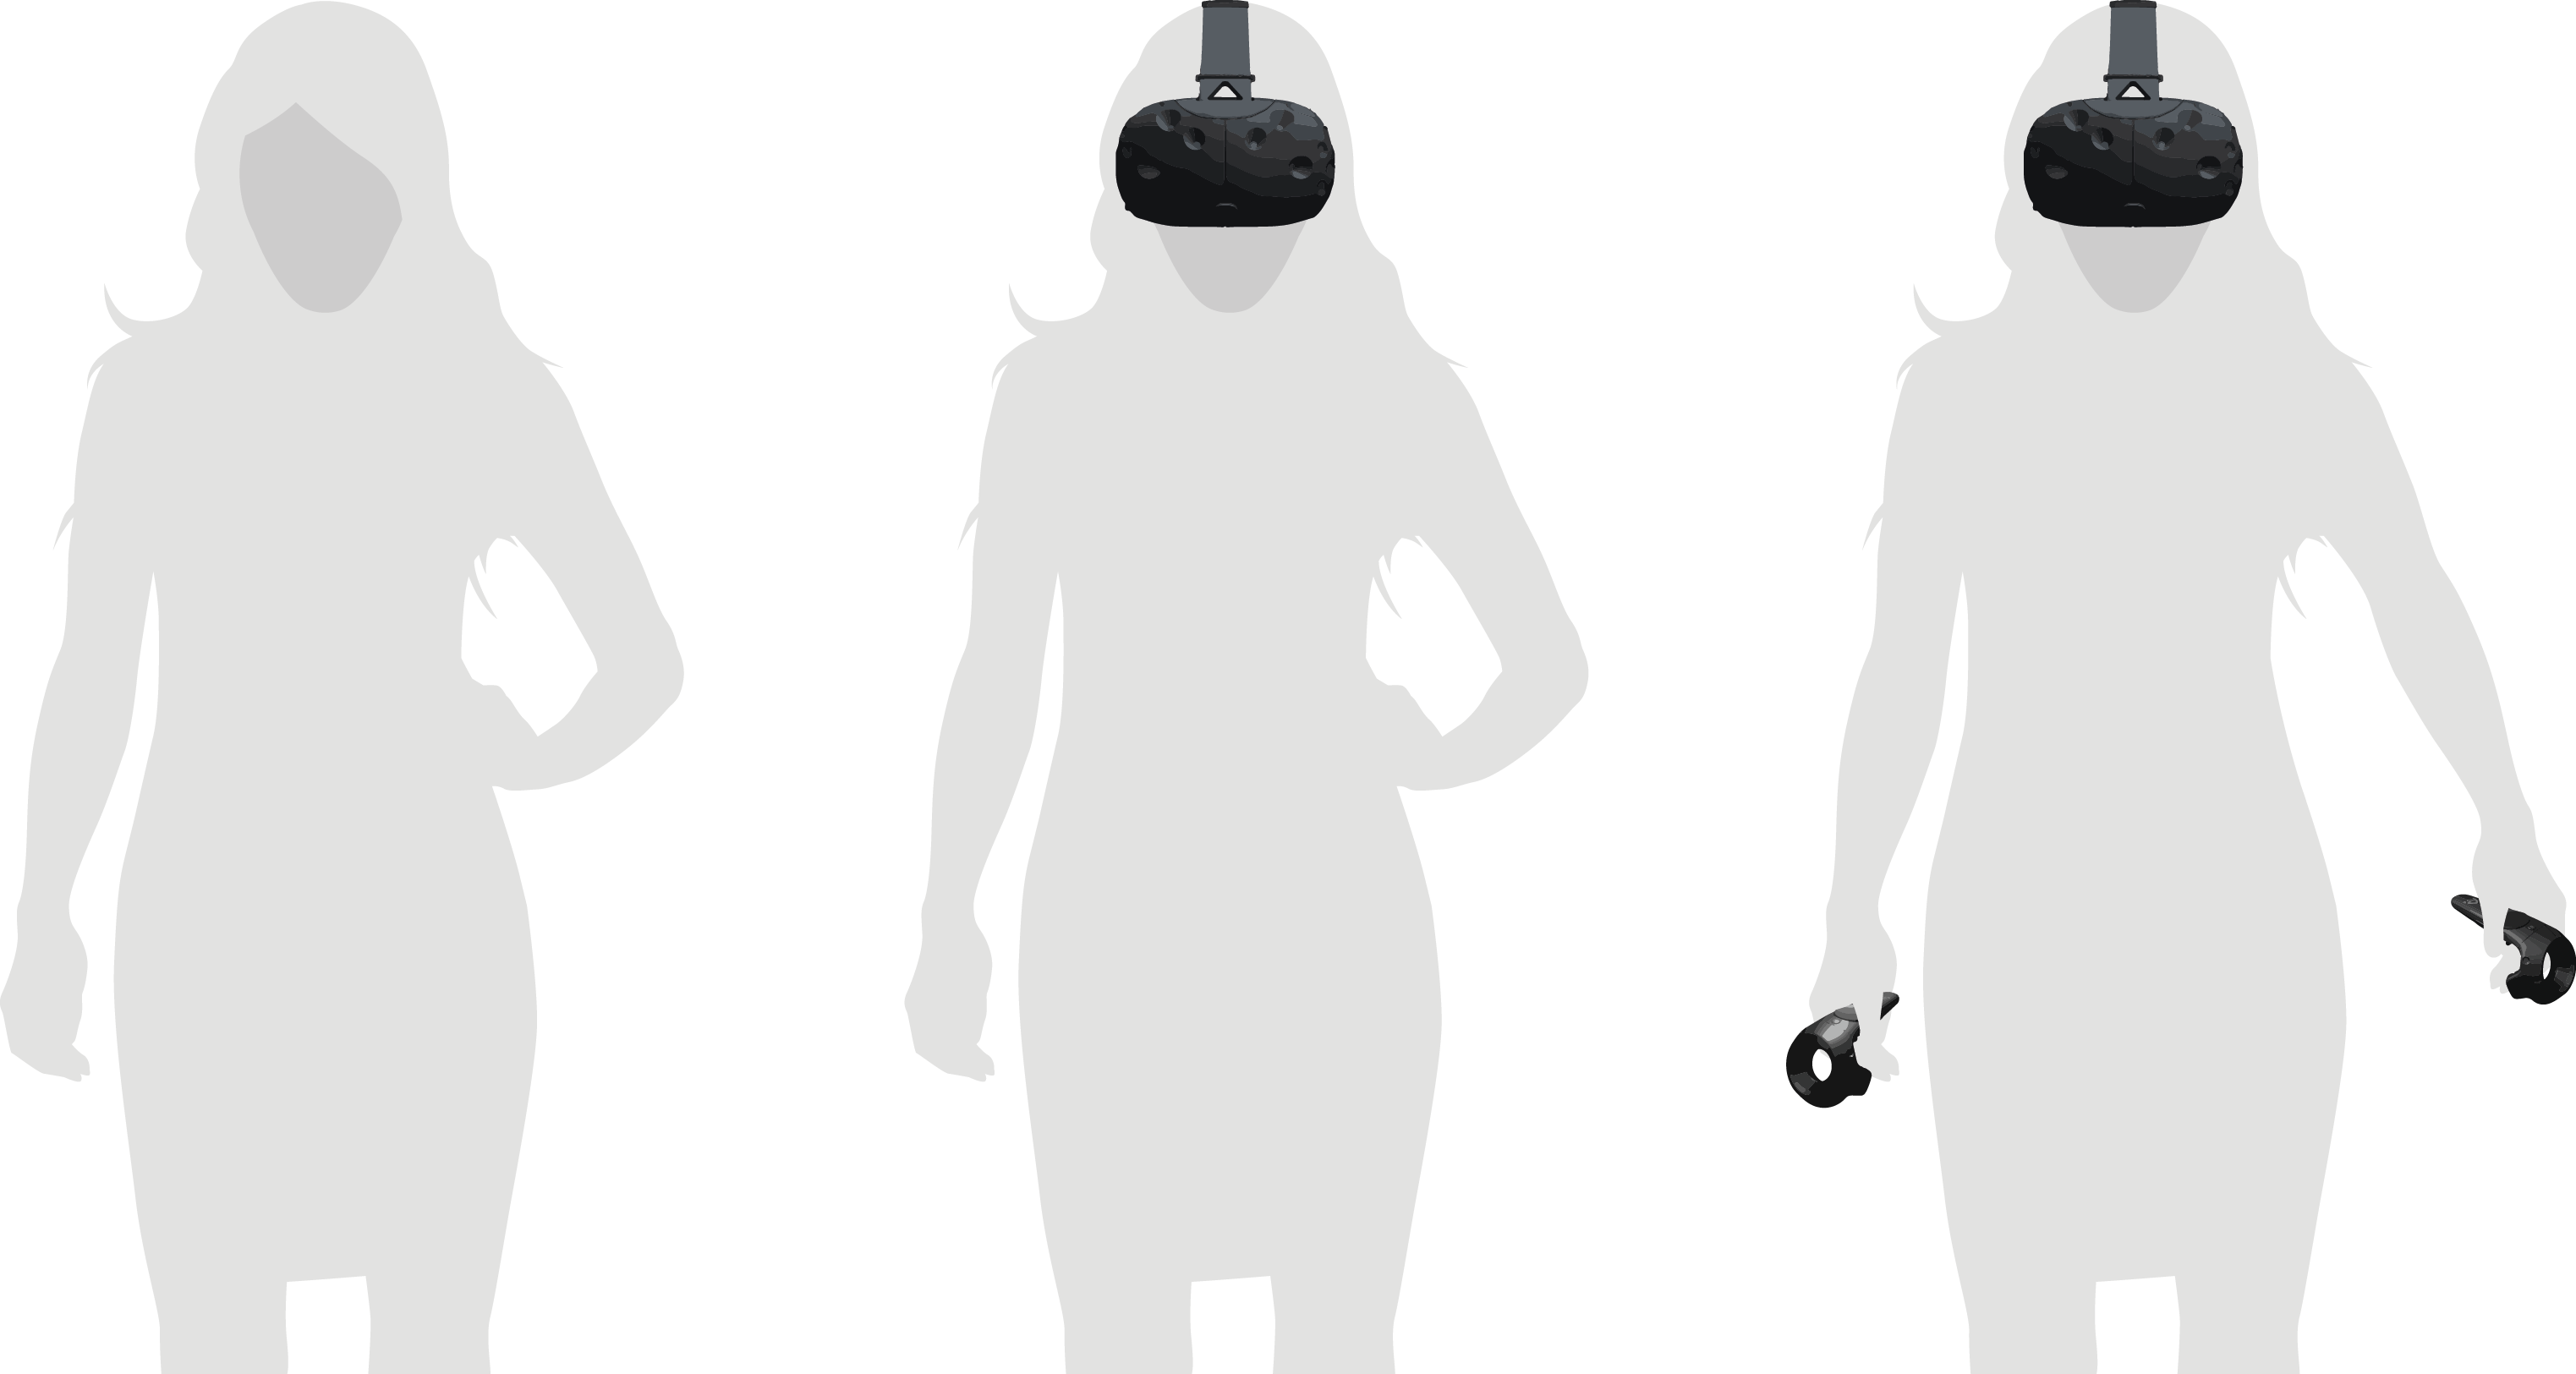
\includegraphics[width=84mm]{female_stimuli.png} 
\caption{Three different female stimuli}
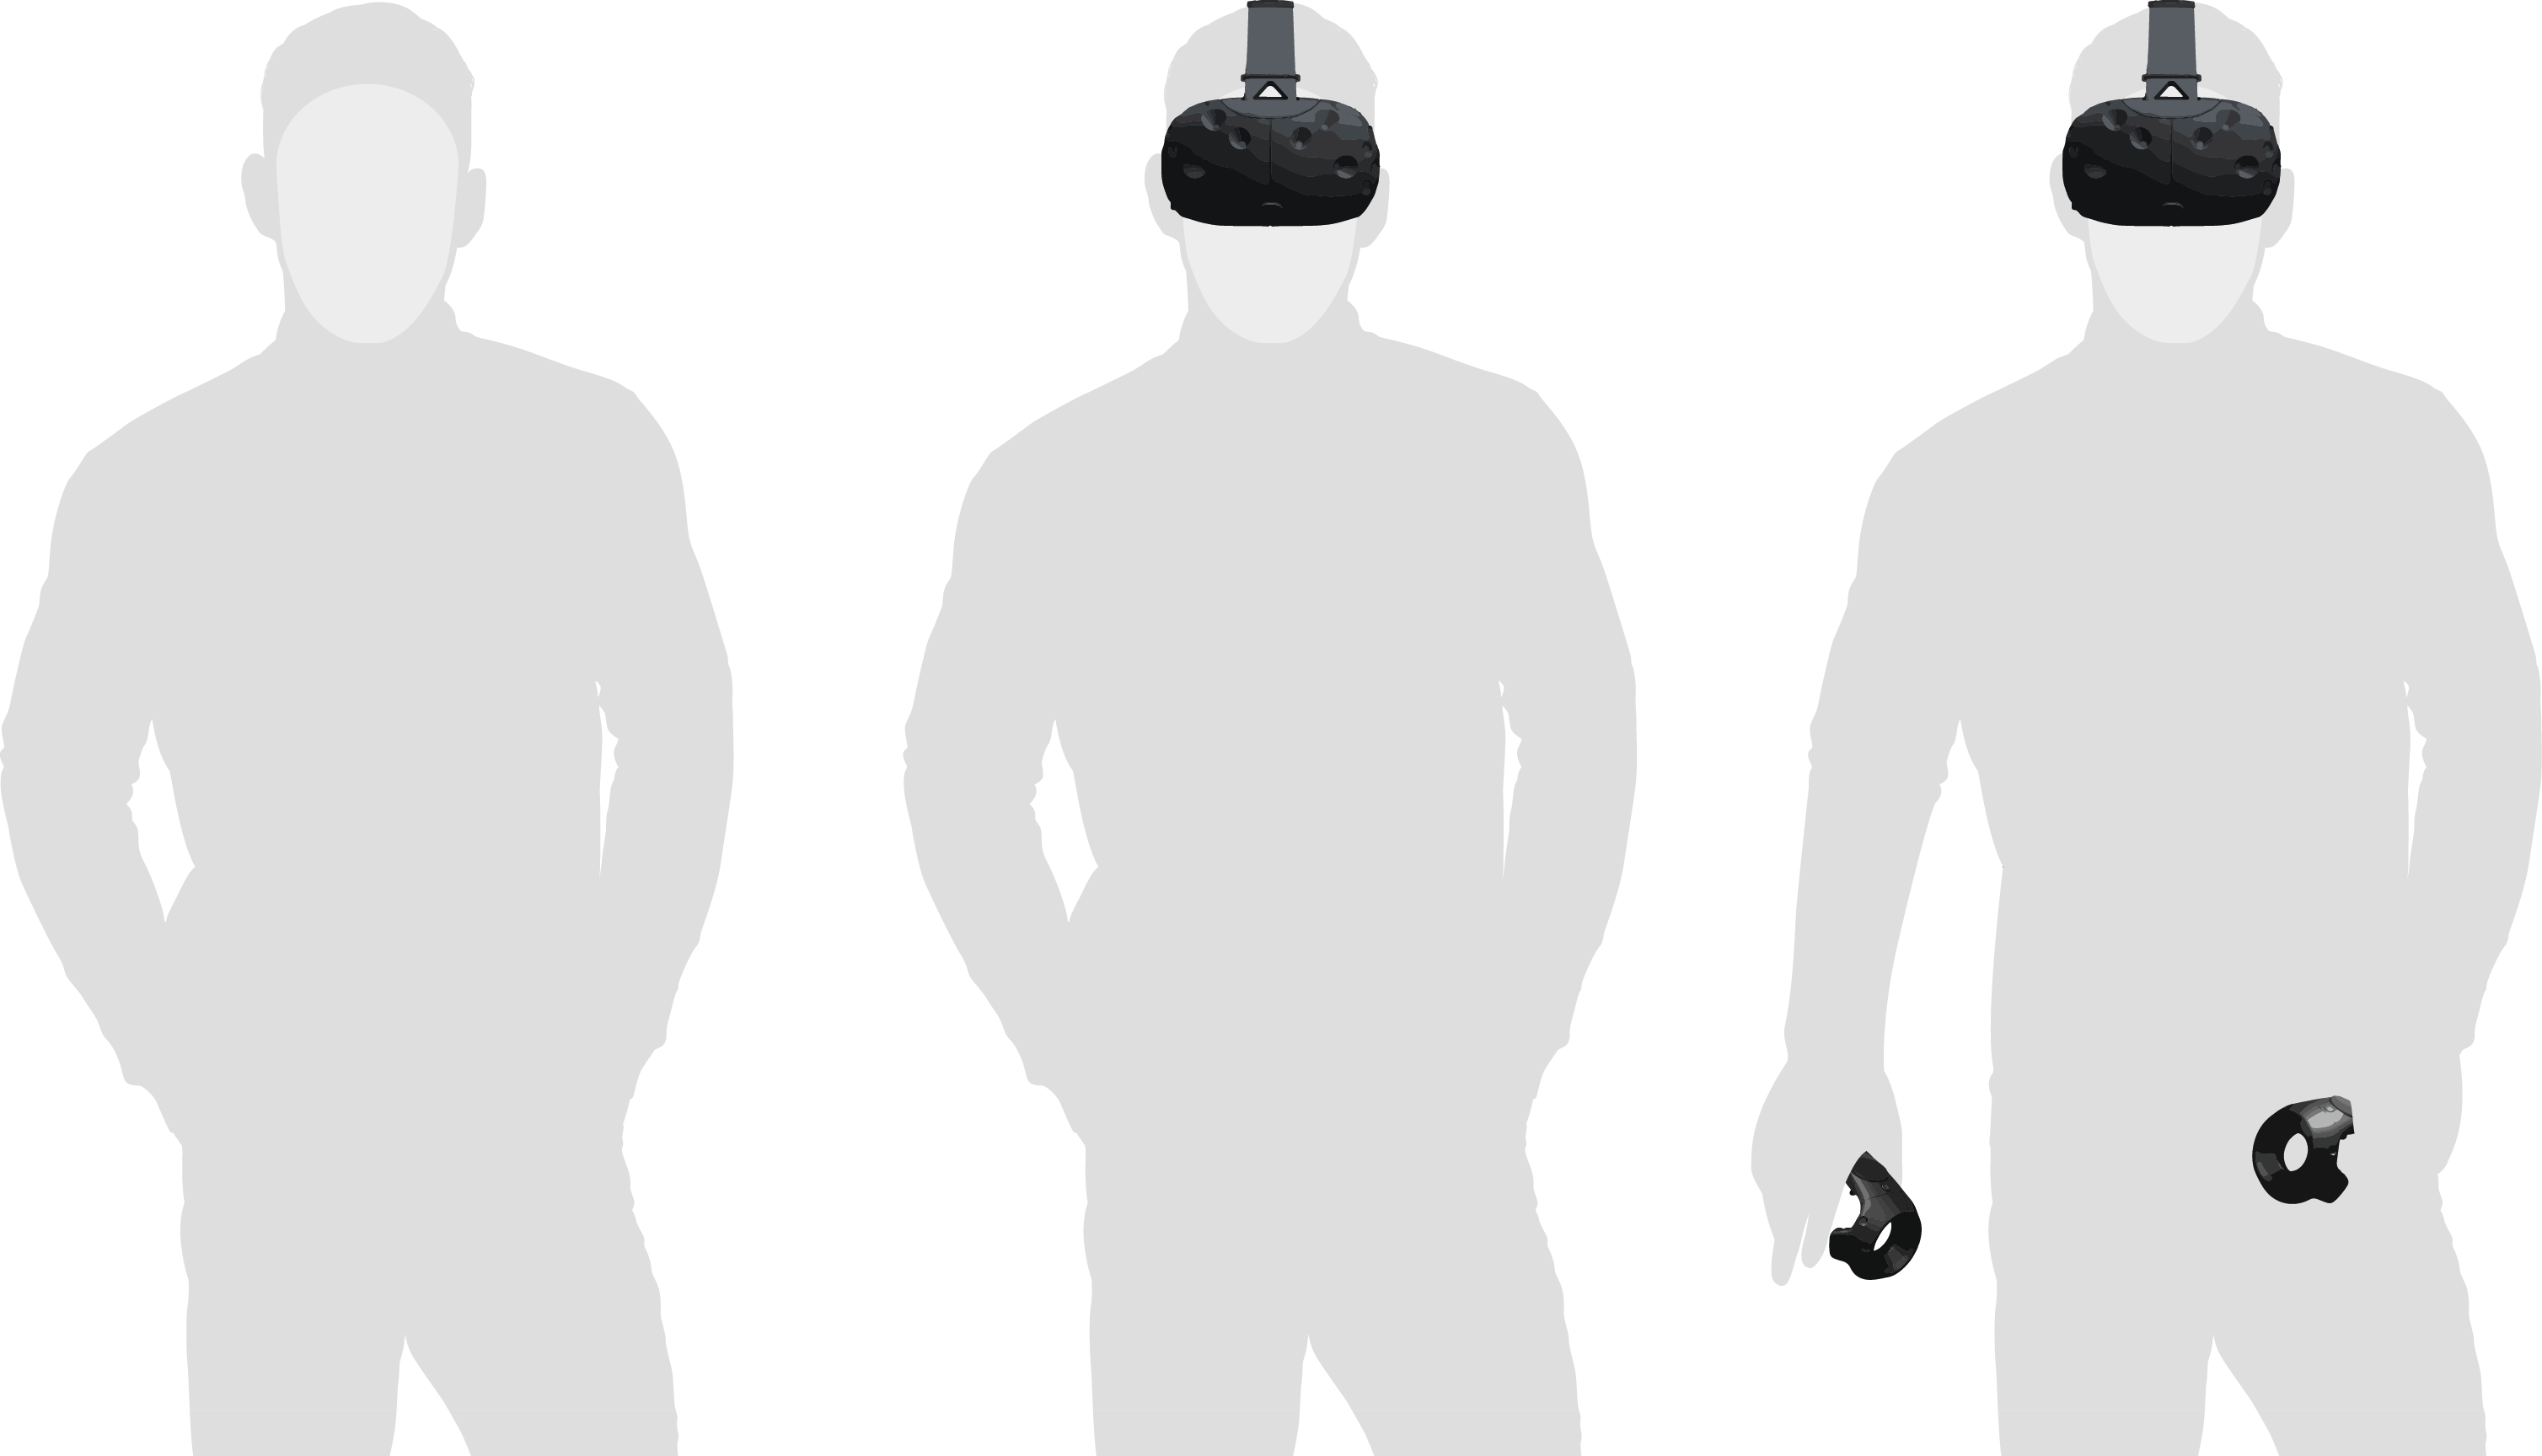
\includegraphics[width=84mm]{male_stimuli.png} 
\caption{Three different male stimuli}
\end{figure}

We wanted to find out if the users gender itself plays an important role in the acceptance of such devices in general. Both genders have been tested without using any VR tools to get a baseline for upcoming steps and procedures, the actors using a smartphone instead for the baseline.
Another stimulus we used was the fact that both our actor and our actress wore a VR goggle to test its influence on the pedestrians.

\begin{figure}[h]
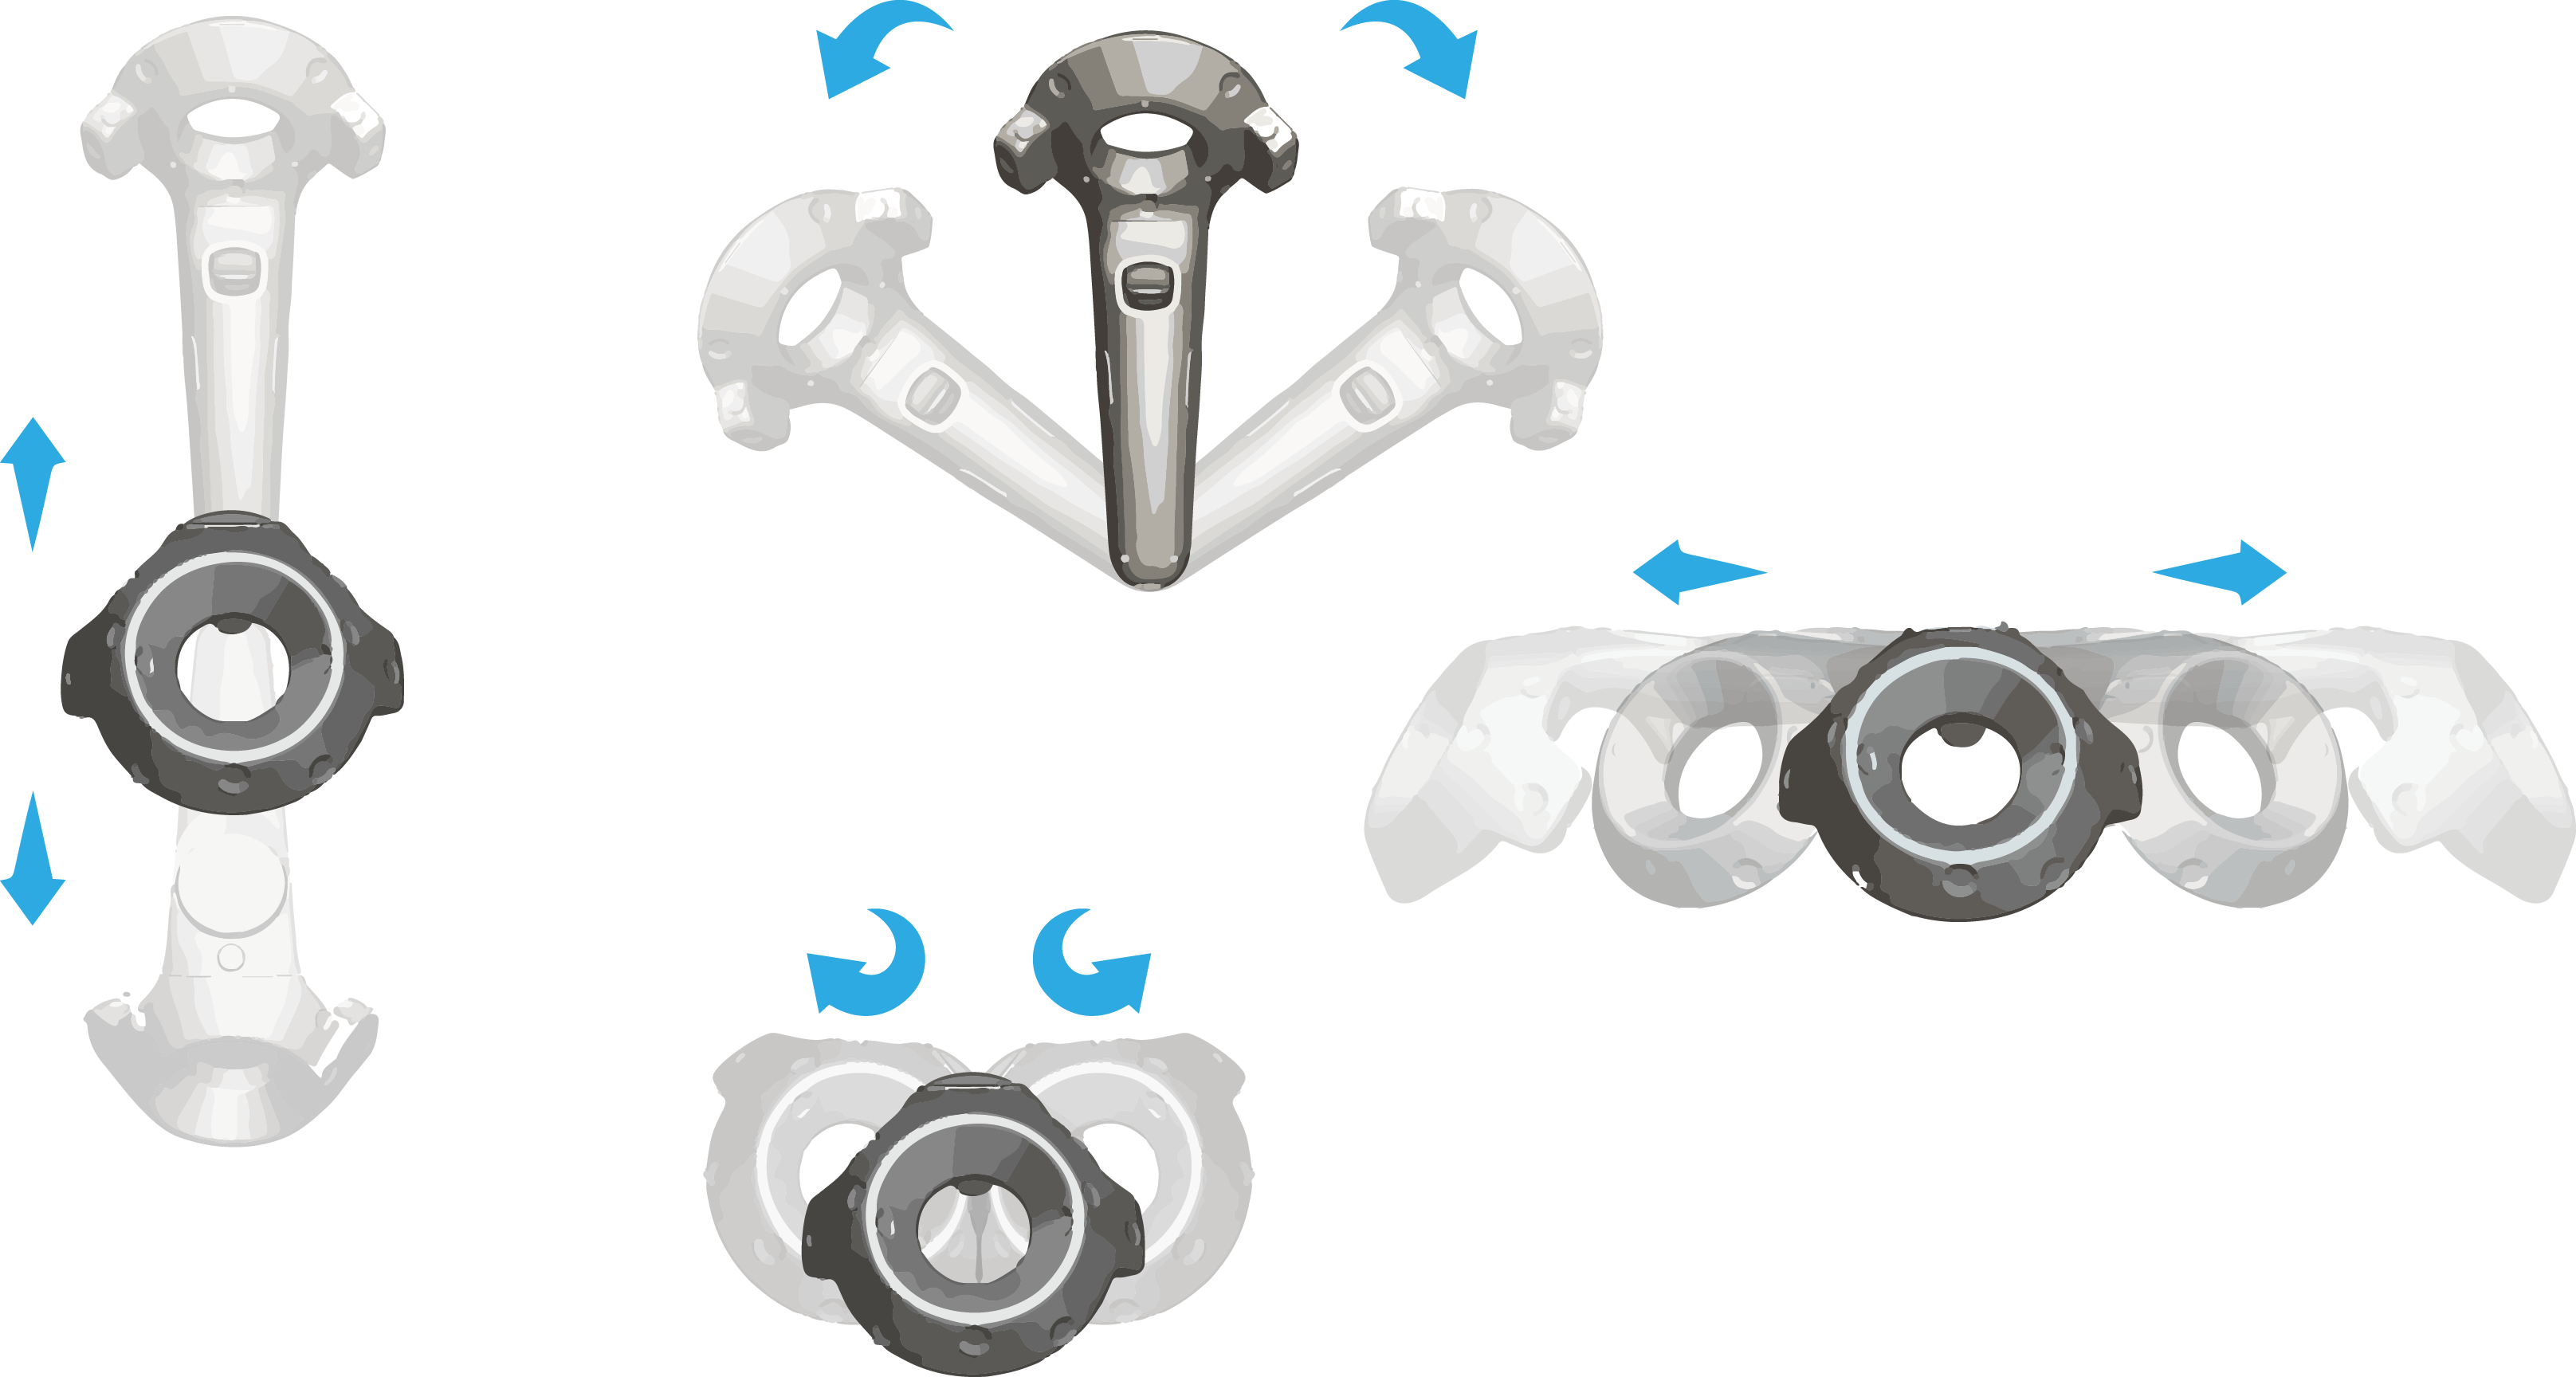
\includegraphics[width=84mm]{vr_gestures.png} 
\caption{Used VR gestures}
\end{figure}

 Last but not least we tested the goggles in combination with controllers and gesture controls which is our final stimulus. In this study we combined those three stimuli to receive as much information as possible about peoples reactions on different types of situations.

\subsection{Survey Procedure}

After handing out the informed consent, the randomly chosen participants answered a short demographic questionaire in which we request allegations to gender and age. Afterwards we handed out another Questionaire to measure the acceptability of wearable devices \cite{kelly2016wear}. After going over the questionnaire with the participants each of them received a little thank-you gift.

\subsection{Participants}

Because this study has not been researched under laboratory conditions it was not possible to recruit test persons. Another reason for us to not hire subjects was, that this would have not lead to the result we were looking for. We wanted to examine this Acceptance Rating by collecting real life reactions and the opinions. For this type of field study it was essential to blindside pedestrians in their daily life to receive an unbiased output. We acquired 60 Participants (33 female, 27 male) for the study. Their age ranged from 19 to 28 (M = 22.65, SD = 2.92).

\section {Results}
An analysis of variance (ANOVA) was conducted to determine the effects of the CASE (mobile phone as control, VR Glasses no gestures, VR-Glasses with gestures) on the AC CEPTABILITY. Statistically significant effects of CASE on DESIRES, a part of theWEAR-Scales overall metric, F = 5.714, p<0.00561, were found. In contrast effects of CASE neither on FEAR nor WEAR revealed any significant results. The effects of the actors gender were also analysed and showed no statistically significant effects either. Due to this t-tests were conducted in pairs between the three CASEs, showing a significant difference between the acceptance of mobile phones and VR-Glasses with the usage of gestures, t = -3.3343, df = 36.391, p-value = 0,001976. Thus results show that the actos gender has no statistically significant impact on the fieldtested CASEs. Solely on DESIRES the CASEs have a significant effect. Significant differences in ACCEPTANCE only exist between smartphone and the wearing of VR glasses while performing gestures.

\section {Mapping and Model}
Using the WEAR scale, data to research acceptance on different wearables can be determined by their relative locations on a 2D map with the dimensions DESIRE and FEAR.

\begin{figure}[h]
\includegraphics[width=84mm]{WEAR-figure.png} 
\caption{Desire-Fear-Plot by CASE and GENDER}
\end{figure}

As one can see in Figure 4 the colored boxes represent the three different cases  (mobile phone as control, VR Glasses no gestures, VR-Glasses with gestures). The dot in the middle of each square locates the mean of the particular case. The box itself shows the horizontal (DESIRES) and vertical (FEARS) variance of the meassurements.
 
\section {Discussion}
The results show only that VR-GLASSES WITH PERFORMING GESTURES reduces the desire of bystanders to be like the user compared to the smartphone using actor, which leads us to the conclussion that there is less bias towards VR-Glasses than one might casually suspect, atleast measurably in a University environment. The significance of these results can be debatable due to the lack of personal background in the form of major or occupation in this study, though we believe it is a proof of concept still, showing that in a neutral public to semi-public environment VR-Glasses can be accepted if no social interaction is expected of the user. The lack of other statistically significant results supports that, though a bigger sample size could reveal different results, if so it stands to reason that the differences in the acceptability of a CASE to the baseline grow more distinct and pronounced, especially with a higher age range, as this study had a rather limited reach there with the ages between 19 and 28. The age, background of the participants and exact setting are probably the biggest factors for the results of a study such as this, be it in the field or in a laboratory. 
Specifically teh performing of gestures warrants extra attention, as this lead to the only significant difference in our study, though not for reasons of social anxiety or simply accidents that could happen when moving your arms and hands in a public environment without seeing, but more from the concext of DESIRE, which leads us to believe that its the self image of the people that would play the biggest role in this regard.

\section {Future Work}
Any future work building on this should prevent the mistakes that were made here first and foremost, the lack of a background in the form or occupation or major in case of students and the proper scaling for the questionnaire just to be comparable with other results delivered by this scale. Past that, a change of setting or variables could deliver a lot more interesting information, be it in a more social setting like a restaurant or cafe, or a more cramped space like most public transport which are both examples of places VR-Devices could get more and more prevalent given time and social acceptance.  Even a repeat of this study in a setting thats not a university could warrant very different results, though we were unable to do that due to issues with permissions a mall would be probably the best space to get sample of most social groups.

%%
%% The next two lines define the bibliography style to be used, and
%% the bibliography file.
\bibliographystyle{ACM-Reference-Format}
\bibliography{sample-base}

%%
%% If your work has an appendix, this is the place to put it.
\appendix
\listoffigures

\end{document}
\endinput
%%
%% End of file `sample-sigchi.tex'.
